%%%%%%%%%%%%%%%%%%%%%%%%%%%%%%%%%%%%%%%%%
% Short Sectioned Assignment LaTeX Template Version 1.0 (5/5/12)
% This template has been downloaded from: http://www.LaTeXTemplates.com
% Original author:  Frits Wenneker (http://www.howtotex.com)
% License: CC BY-NC-SA 3.0 (http://creativecommons.org/licenses/by-nc-sa/3.0/)
%%%%%%%%%%%%%%%%%%%%%%%%%%%%%%%%%%%%%%%%%

%----------------------------------------------------------------------------------------
%	PACKAGES AND OTHER DOCUMENT CONFIGURATIONS
%----------------------------------------------------------------------------------------

\documentclass[paper=a4, fontsize=11pt]{scrartcl} % A4 paper and 11pt font size

% ---- Entrada y salida de texto -----

\usepackage[T1]{fontenc} % Use 8-bit encoding that has 256 glyphs
\usepackage[utf8]{inputenc}
%\usepackage{fourier} % Use the Adobe Utopia font for the document - comment this line to return to the LaTeX default

% ---- Idioma --------

\usepackage[spanish, es-tabla]{babel} % Selecciona el español para palabras introducidas automáticamente, p.ej. "septiembre" en la fecha y especifica que se use la palabra Tabla en vez de Cuadro

% ---- Otros paquetes ----

\usepackage[hidelinks]{hyperref} % Estilo para los enlaces
\hypersetup{
  colorlinks   = true, %Colours links instead of ugly boxes
  urlcolor     = blue, %Colour for external hyperlinks
  linkcolor    = black, %Colour of internal links
  citecolor   = blue %Colour of citations
}
\usepackage{url} % ,href} %para incluir URLs e hipervínculos dentro del texto (aunque hay que instalar href)
\usepackage{amsmath,amsfonts,amsthm} % Math packages
%\usepackage{graphics,graphicx, floatrow} %para incluir imágenes y notas en las imágenes
\usepackage{graphics,graphicx, float} %para incluir imágenes y colocarlas
\usepackage{eurosym}

% Para hacer tablas comlejas
%\usepackage{multirow}
%\usepackage{threeparttable}

%\usepackage{sectsty} % Allows customizing section commands
%\allsectionsfont{\centering \normalfont\scshape} % Make all sections centered, the default font and small caps

\usepackage{fancyhdr} % Custom headers and footers
\pagestyle{fancyplain} % Makes all pages in the document conform to the custom headers and footers
\fancyhead{} % No page header - if you want one, create it in the same way as the footers below
\fancyfoot[L]{} % Empty left footer
\fancyfoot[C]{} % Empty center footer
\fancyfoot[R]{\thepage} % Page numbering for right footer
\renewcommand{\headrulewidth}{0pt} % Remove header underlines
\renewcommand{\footrulewidth}{0pt} % Remove footer underlines
\setlength{\headheight}{13.6pt} % Customize the height of the header

\numberwithin{equation}{section} % Number equations within sections (i.e. 1.1, 1.2, 2.1, 2.2 instead of 1, 2, 3, 4)
\numberwithin{figure}{section} % Number figures within sections (i.e. 1.1, 1.2, 2.1, 2.2 instead of 1, 2, 3, 4)
\numberwithin{table}{section} % Number tables within sections (i.e. 1.1, 1.2, 2.1, 2.2 instead of 1, 2, 3, 4)

\setlength\parindent{0pt} % Removes all indentation from paragraphs - comment this line for an assignment with lots of text

\newcommand{\horrule}[1]{\rule{\linewidth}{#1}} % Create horizontal rule command with 1 argument of height


%----------------------------------------------------------------------------------------
%	TÍTULO Y DATOS DEL ALUMNO
%----------------------------------------------------------------------------------------

\title{	
\normalfont \normalsize 
\textsc{\textbf{Ingeniería de Servidores (2016-2017)} \\ Grado en Ingeniería Informática \\ Universidad de Granada} \\ [25pt] % Your university, school and/or department name(s)
\horrule{0.5pt} \\[0.4cm] % Thin top horizontal rule
\huge Memoria Práctica 5 \\ % The assignment title
\horrule{2pt} \\[0.5cm] % Thick bottom horizontal rule
}

\author{Elena María Gómez Ríos} % Nombre y apellidos

\date{\normalsize\today} % Incluye la fecha actual

%----------------------------------------------------------------------------------------
% DOCUMENTO
%----------------------------------------------------------------------------------------

\begin{document}

\maketitle % Muestra el Título

\newpage %inserta un salto de página

\tableofcontents % para generar el índice de contenidos

\listoffigures

\listoftables

\newpage

%\textbf{NOTA: en caso de problema al compilar, compruebe que tiene el paquete: texlive-babel-spanish.noarch }  \\
 


\newpage

%----------------------------------------------------------------------------------------
%	Cuestión 1
%----------------------------------------------------------------------------------------

\section{Cuestión 1:}

\subsection{Al modificar los valores del kernel de este modo, no logramos que persistan después de reiniciar la máquina. ¿Qué archivo hay que editar para que los cambios sean permanentes?}

Tal y como se indica en \cite{sysctl}, para que las modificaciones realizadas persistan después de reiniciar la máquina se debe editar el archivo de configuración de sysctl, \texttt{/etc/sysctl.conf}. El contenido de dicho archivo por defecto se puede ver en la figura \ref{fig:ejercicio1_1}. Para cargar el cambio realizado sin tener que reiniciar el sistema se usa el comando \texttt{sysctl ­-p}.\\

Por ejemplo he listado los valores de sysctl con la orden sysctl -a (figura \ref{fig:ejercicio1_2}) y he cambiado uno de los valores para comprobar que funcionaba correctamente (figuras \ref{fig:ejercicio1_3}, \ref{fig:ejercicio1_4} y \ref{fig:ejercicio1_5}).

\begin{figure}[H] 
	\centering
	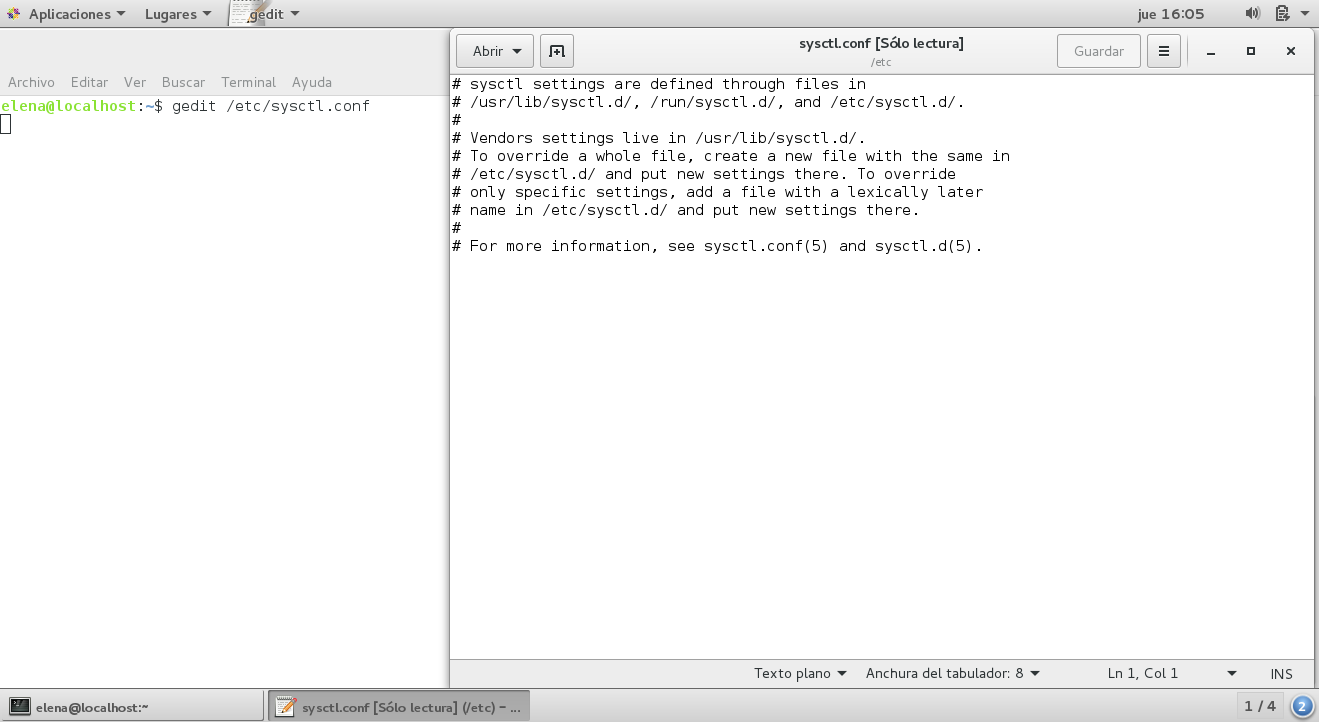
\includegraphics[width=14.7cm]{./img/ejercicio1_1.png} 	
	\caption{CentOS, contenido del archivo sysctl.conf.} \label{fig:ejercicio1_1}
\end{figure}

\begin{figure}[H] 
	\centering
	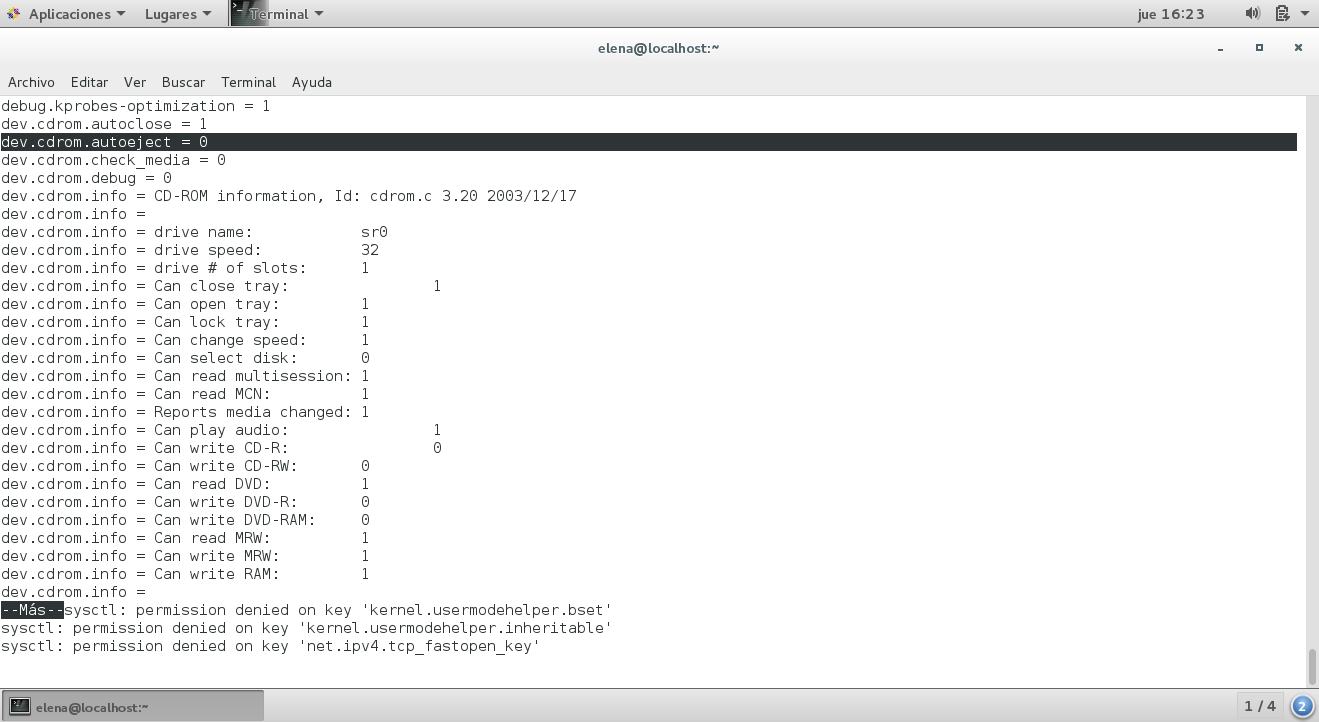
\includegraphics[width=14.7cm]{./img/ejercicio1_2.png} 	
	\caption{CentOS, salida de sysctl -a antes de la modificación.} \label{fig:ejercicio1_2}
\end{figure}

\begin{figure}[H] 
	\centering
	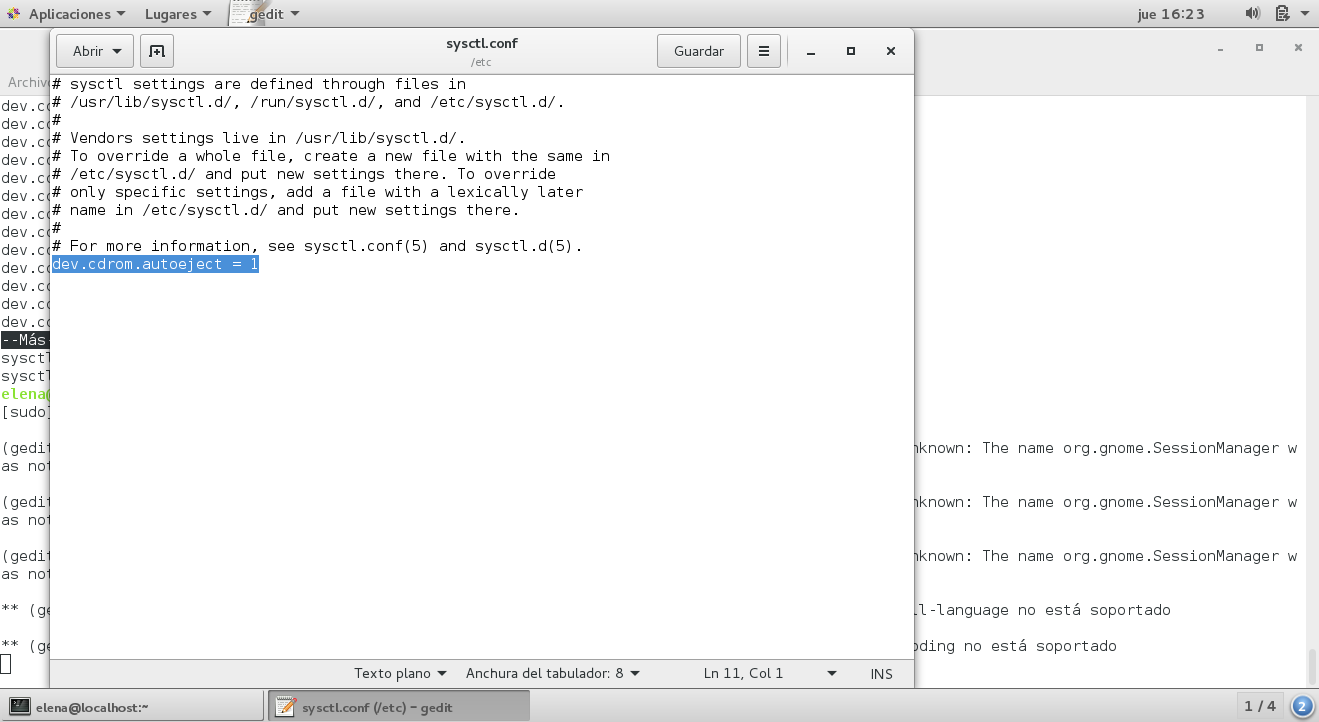
\includegraphics[width=14.7cm]{./img/ejercicio1_3.png} 	
	\caption{CentOS, modificación del archivo sysctl.conf.} \label{fig:ejercicio1_3}
\end{figure}

\begin{figure}[H] 
	\centering
	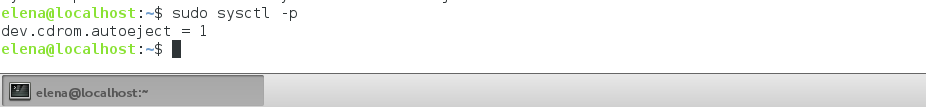
\includegraphics[width=10cm]{./img/ejercicio1_4.png} 	
	\caption{CentOS, comando sysctl -p.} \label{fig:ejercicio1_4}
\end{figure}

\begin{figure}[H] 
	\centering
	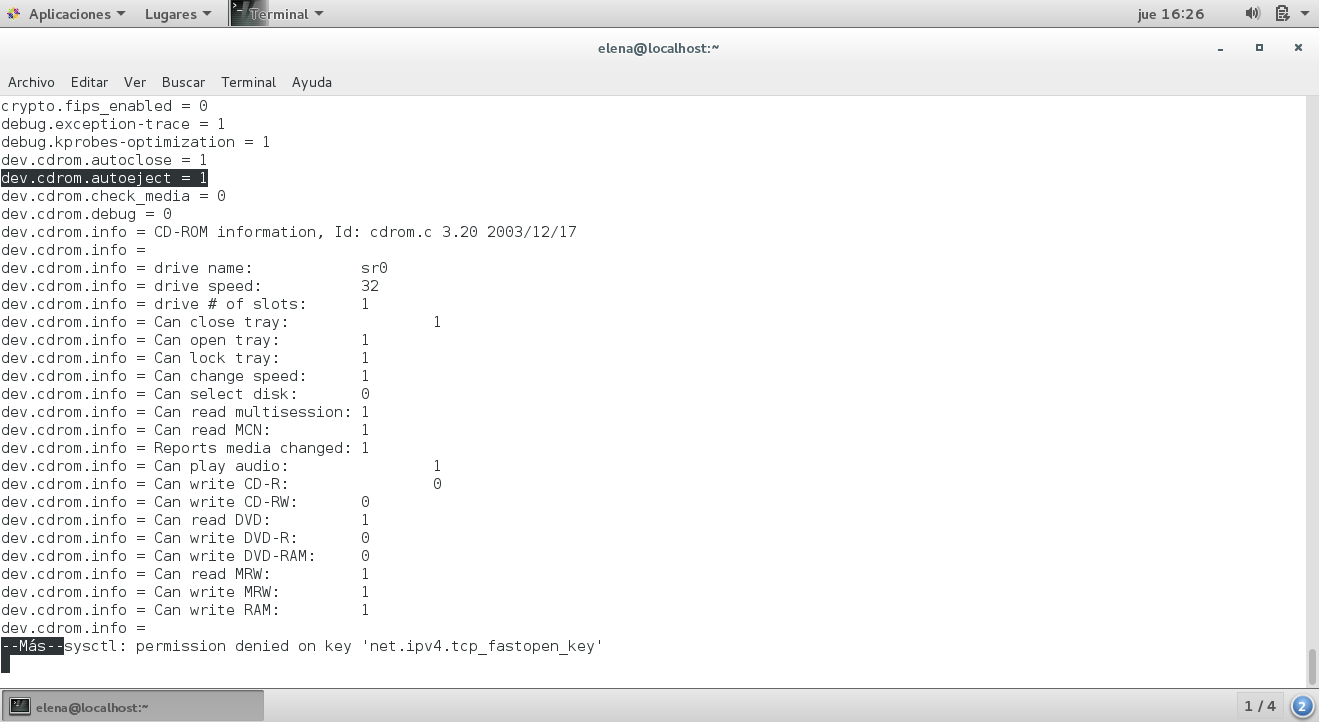
\includegraphics[width=13cm]{./img/ejercicio1_5.png} 	
	\caption{CentOS,  salida de sysctl -a después de la modificación.} \label{fig:ejercicio1_5}
\end{figure}


%----------------------------------------------------------------------------------------
%	Cuestión 2
%----------------------------------------------------------------------------------------

\section{Cuestión 2:}

\subsection{¿Con qué opción se muestran todos los parámetros modificables en tiempo de ejecución? Elija dos parámetros y explique, en dos líneas, qué función tienen.}
Tal y como se indica en el manual de \texttt{sysctl} la opción con la que se muestran todos los parámetros modificables en tiempo de ejecución es \texttt{sysctl -a} (figura \ref{fig:ejercicio1_2}). \\

Los parámetros del sistema se encuentran dentro de \texttt{/proc/sys/}. Como se puede observar en la documentación de Red Hat \cite{ejer2}, por ejemplo el parámetro \texttt{kernel.threads-max} establece el número máximo de hilos o hebras que se pueden ejecutar en el sistema, el parámetro \texttt{kernel.pid­max} establece el número máximo de PID que puede ser asignado a un proceso o hebra, o el parámetro \texttt{kernel.msgmax} el cual define el tamaño máximo permitido en bytes de cualquier mensaje individual en una cola de mensajes.


%----------------------------------------------------------------------------------------
%	Cuestión 3
%----------------------------------------------------------------------------------------

\section{Cuestión 3:}

\subsection{a) Realice una copia de seguridad del registro y restáurela, ilustre el proceso con capturas.}

Para realizar una copia de seguridad del registro entramos en \texttt{regedit} y seleccionamos ``Exportar...'' dentro de ``Archivo'', como se muestra en la figura \ref{fig:ejercicio3_1}. Se nos abrirá una ventana en la cual se pedirá el lugar donde queremos guardar la copia de seguridad, un nombre y si queremos una copia de todo el registro o sólo de la rama seleccionada, en nuestro caso selecciono todo el registro (figura \ref{fig:ejercicio3_2}).\\

Para restaurarla accedemos al ``Editor del registro'' y en la pestaña ``Archivo'' seleccionamos ``Importar...'' (figura \ref{fig:ejercicio3_3}). Se nos abrirá una ventana en la cual seleccionamos la copia de seguridad que queremos restaurar (figura \ref{fig:ejercicio3_4}).\\

Como se puede observar en la página de Microsoft \cite{ejer3} para realizar la copia de seguridad del registro hay que seguir los pasos que he realizado en el ejercicio. En dicha documentación también se explica como hacer y restaurar una copia de seguridad del sistema, pero entiendo que esto no es lo que se pide en este ejercicio.

\begin{figure}[H] 
	\centering
	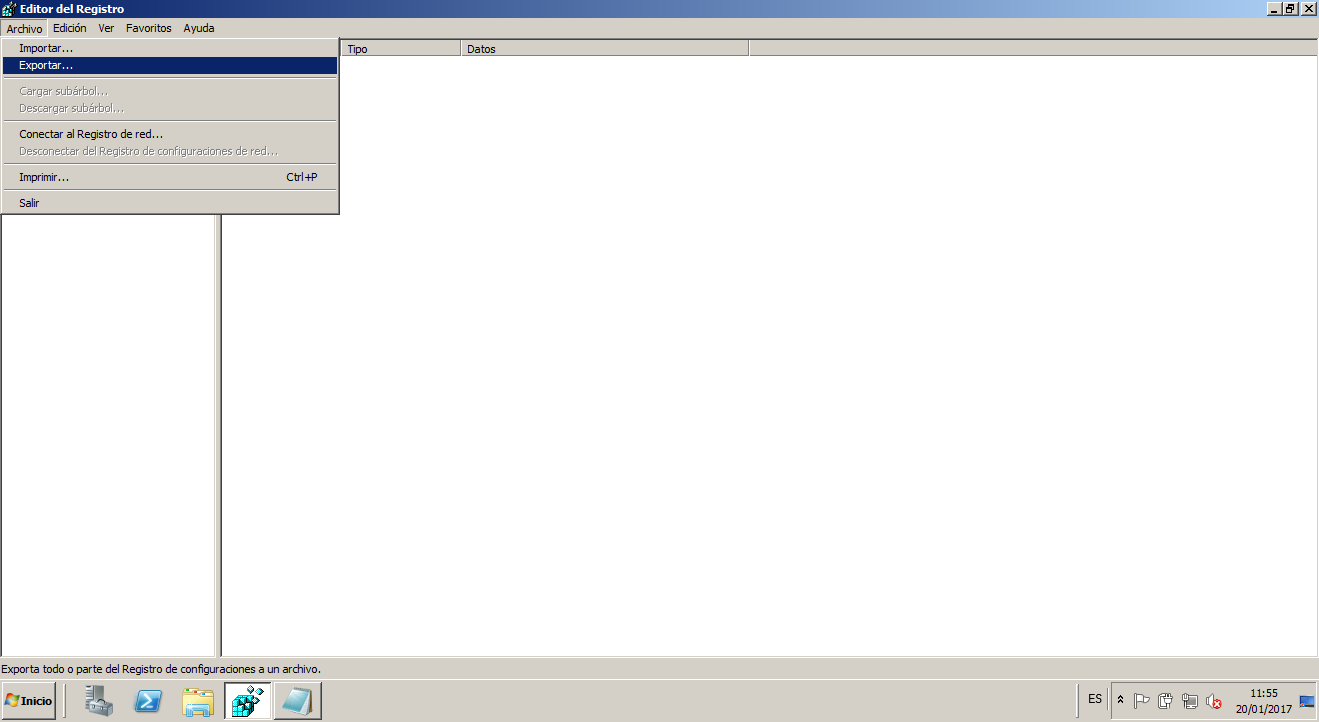
\includegraphics[width=14.7cm]{./img/ejercicio3_1.png} 	
	\caption{Windows, editor del registro.} \label{fig:ejercicio3_1}
\end{figure}

\begin{figure}[H] 
	\centering
	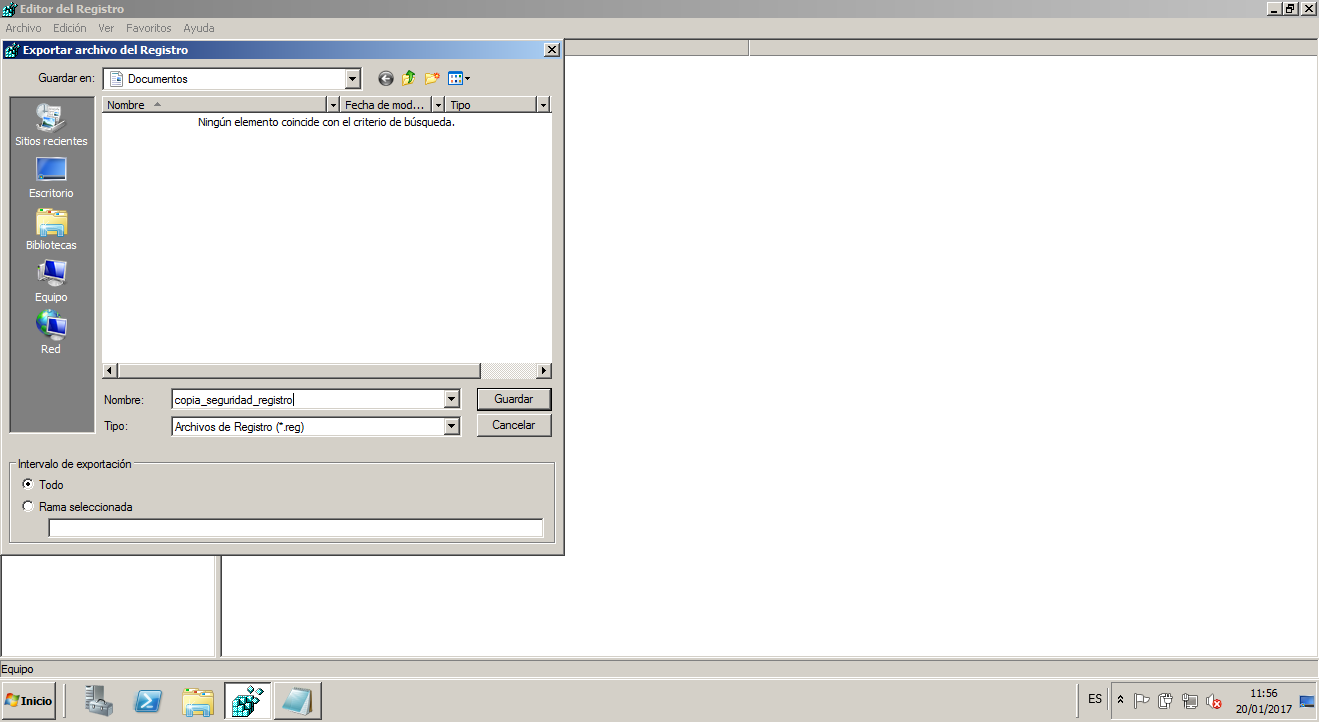
\includegraphics[width=14.7cm]{./img/ejercicio3_2.png} 	
	\caption{Windows, editor del registro, copia de seguridad.} \label{fig:ejercicio3_2}
\end{figure}

\begin{figure}[H] 
	\centering
	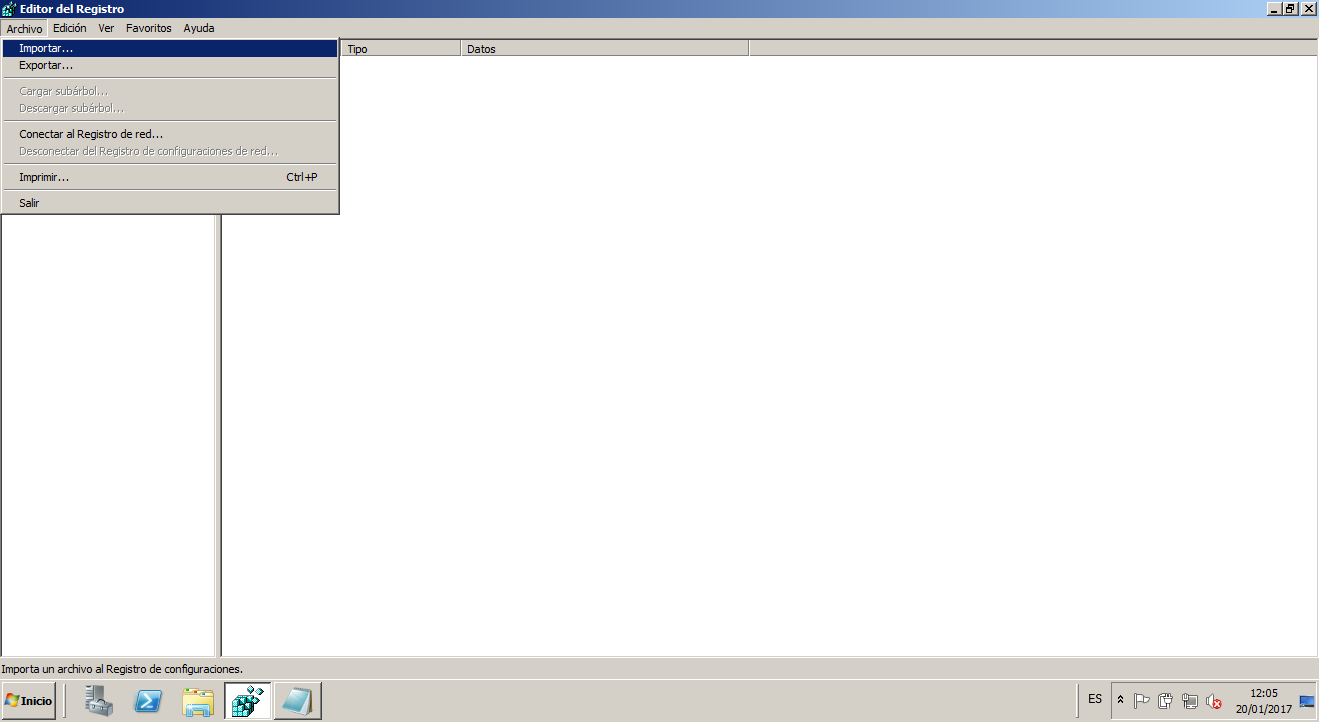
\includegraphics[width=14.7cm]{./img/ejercicio3_3.png} 	
	\caption{Windows, editor del registro, restauar copia de seguridad.} \label{fig:ejercicio3_3}
\end{figure}

\begin{figure}[H] 
	\centering
	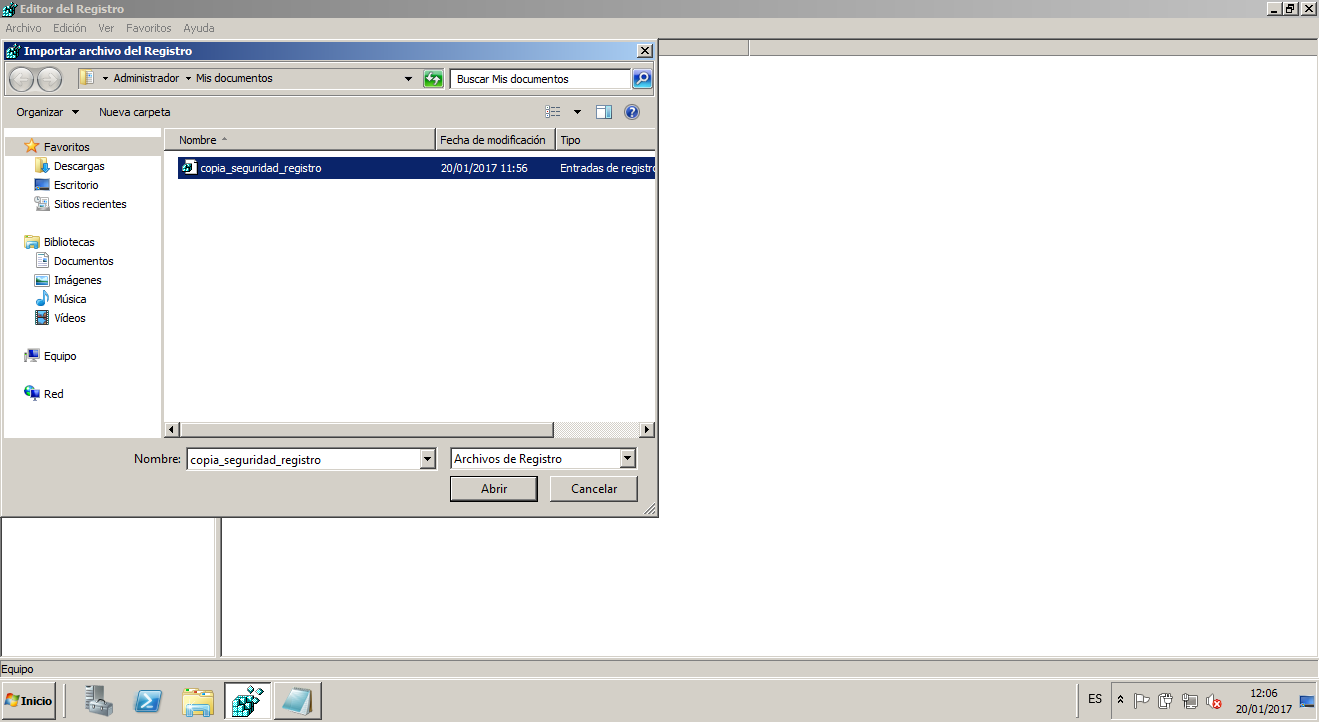
\includegraphics[width=14.7cm]{./img/ejercicio3_4.png} 	
	\caption{Windows, editor del registro, restauar copia de seguridad.} \label{fig:ejercicio3_4}
\end{figure}


\subsection{b) Abra una ventana mostrando el editor del registro.}
El editor del registro se puede ver en el apartado anterior (figura \ref{fig:ejercicio3_1})



%----------------------------------------------------------------------------------------
%	Cuestión 4
%----------------------------------------------------------------------------------------

\section{Cuestión 4:}

\subsection{Enumere qué elementos se pueden configurar en Apache y en IIS para que Moodle funcione mejor.}

Como se dice en el guión de prácticas en \cite{ejer4} se encuentran algunos consejos de la configuración de \texttt{Apache} e \texttt{IIS} para que \texttt{Moodle} funcione mejor.\\

Las configuraciones recomendadas para Apache son: 
\begin{itemize}
	\item Establecer un número máximo de clientes (parámetro \texttt{MaxClients}) calculando el 80\% de la memoria total disponible y dividiendo por el máximo uso de memoria de un proceso de Apache.  
	\item Reducir el número de módulos que Apache carga en el archivo \texttt{httpd.conf} para  minimizar el uso de memoria.
	\item Usar la última versión de Apache.
	\item En los sistemas Linux/Unix establecer el máximo número de hijos por proceso a 20-­30 (parámetro \texttt{MaxRequestsPerChild} en in \texttt{httpd.conf}).
	\item En los servidores con mucha carga, establecer \texttt{KeepAlive} a \texttt{off} o disminuir el parámetro \texttt{KeepAliveTimeout} entre 2 y 5.
	\item Si no se usa un fichero \texttt{.htaccess} establecer la variable \texttt{AllowOverride} a \texttt{None}.
	\item Establecer el \texttt{DirectoryIndex} de forma correcta.
	\item Establecer \texttt{ExtendedStatus} a \texttt{Off} y desactivar tanto \texttt{mod\_info} como \texttt{mod\_status}.
	\item Dejar el \texttt{HostnameLookups} a su valor por defecto, \texttt{Off}, para reducir la latencia de \texttt{DNS}.
	\item Reducir el valor de \texttt{TimeOut} a 30-60 segundos.
\end{itemize}

Las configuraciones recomendadas para IIS son: 
\begin{itemize}
	\item Cambiar \texttt{ListenBackLog} a un valor entre 2 y 5.
	\item Cambiar el valor \texttt{MemCacheSize} para ajustar la cantidad de memoria que \texttt{IIS} usará para su archivo caché.
	\item Cambiar el parámetro \texttt{MaxCachedFileSize} para ajustar el tamaño máximo de un archivo situado en la memoria caché. Por defecto es 262,144 (256K).
	\item Crear un nuevo \texttt{DWORD} llamado \texttt{ObjectCacheTTL} para cambiar el tiempo que los objetos se mantienen en la memoria caché.
\end{itemize}



%----------------------------------------------------------------------------------------
%	Cuestión 5
%----------------------------------------------------------------------------------------

\section{Cuestión 5:}
\subsection{Ajuste la compresión en el servidor y analice su comportamiento usando varios valores para el tamaño de archivo a partir del cual comprimir. Para comprobar que está comprimiendo puede usar el navegador o comandos como curl (see url) o lynx. Muestre capturas de pantalla de todo el proceso.}

Para habilitar la compresión en el servidor accedemos al ``Administrador de Internet Information Services IIS'', seleccionamos la opción de compresión (figura \ref{fig:ejercicio5_2}), en la cual podemos habilitar la comprensión y elegir el tamaño mínimo a partir del cual se va a empezar a comprimir. En mi caso he cambiado dicho tamaño a 250 como se muestra en la figura \ref{fig:ejercicio5_4}.\\

Para comprobar que funciona accedemos a la página desde el navegador, y desde el propio navegador podemos ver el tamaño de la página (figura \ref{fig:ejercicio5_1}), también podemos ver las características y comprobar que acepta la codificación gzip (figura \ref{fig:ejercicio5_3}). \\

Por último otra forma de comprobar el funcionamiento de la compresión es utilizar curl el cual se puede descargar de su página oficial \cite{curl}. Una vez descargado simplemente tenemos que introducir en la consola de Windows: \texttt{curl -I -H 'Accept-Encoding: gzip' http://localhost'} el cual nos muestra las mismas características que aparecían en Chrome.\\

Como se puede apreciar en las capturas no he conseguido realizar la compresión de forma correcta aunque he seguido todos los pasos descritos. He estado varias horas intentando encontrar el error, ya fuese de configuración del IIS o algún tipo de problema en mi máquina, pero no he conseguido encontrar donde puede estar el error. 

\begin{figure}[H] 
	\centering
	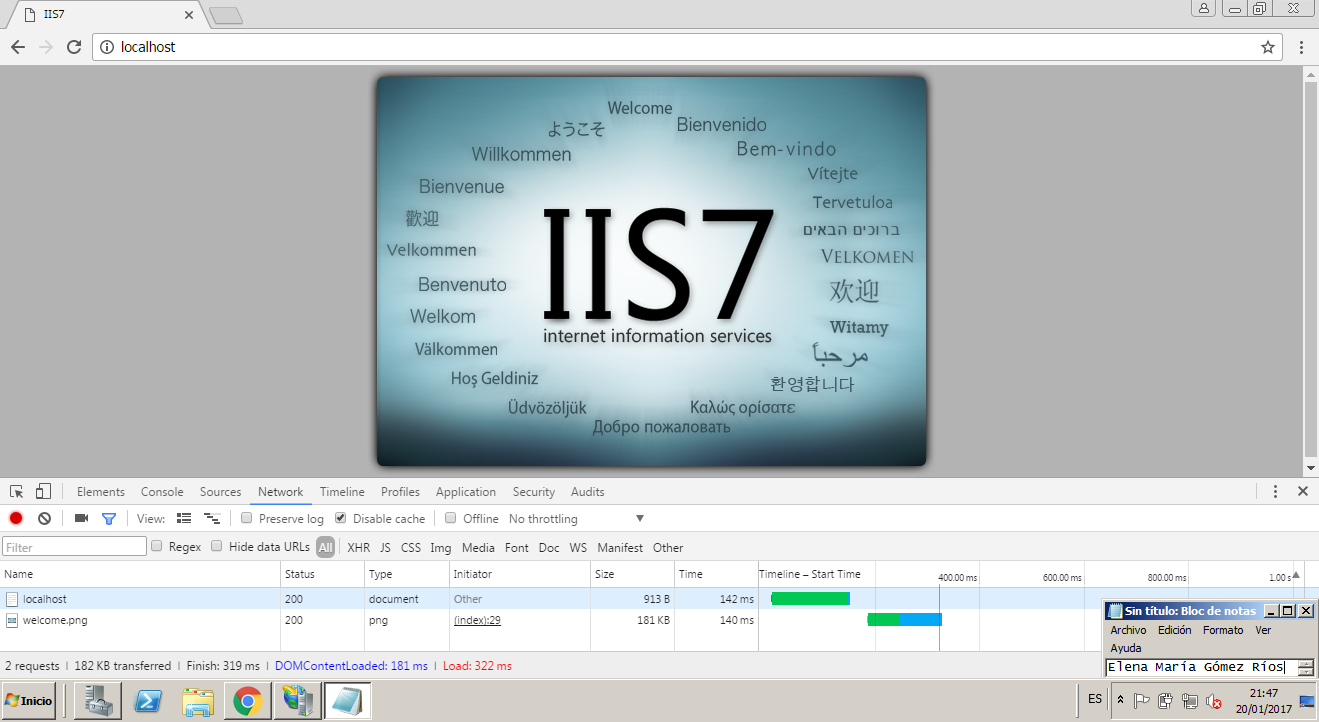
\includegraphics[width=14.7cm]{./img/ejercicio5_1.png} 	
	\caption{Windows, opciones de Network de Chrome.} \label{fig:ejercicio5_1}
\end{figure}

\begin{figure}[H] 
	\centering
	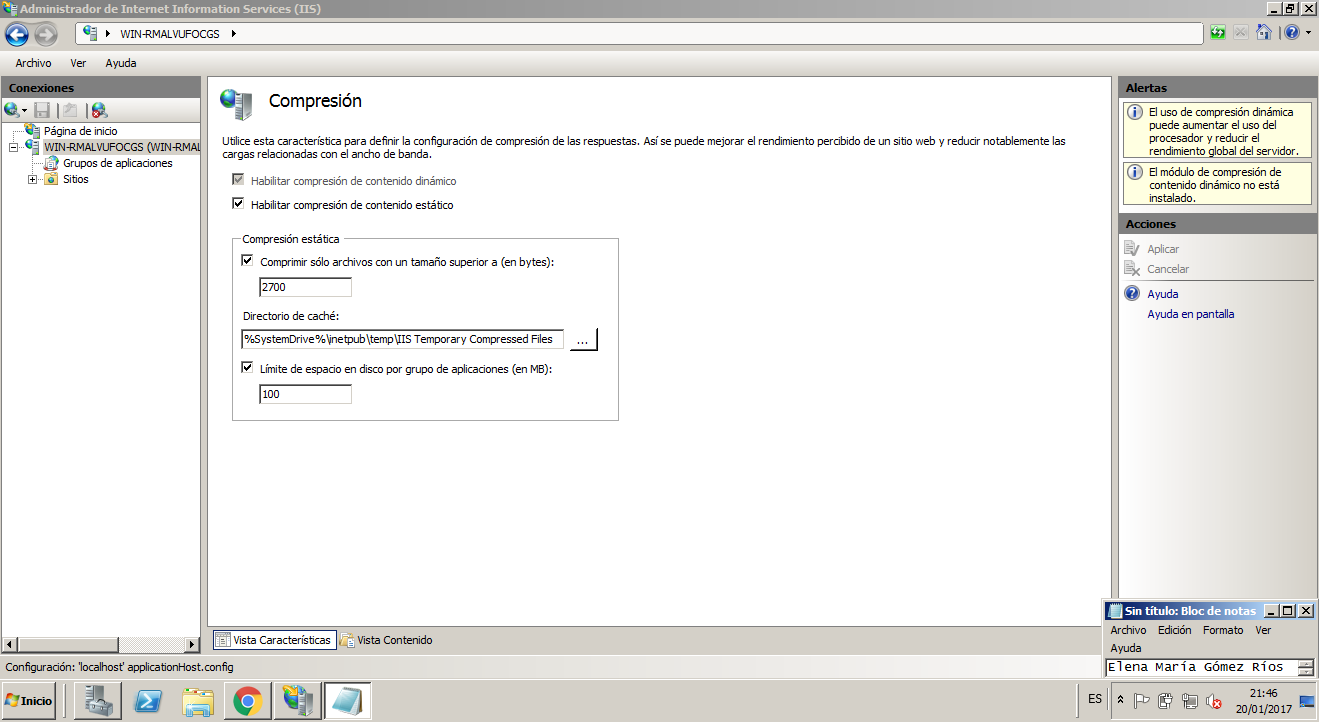
\includegraphics[width=14.7cm]{./img/ejercicio5_2.png} 	
	\caption{Windows, configuración de compresión.} \label{fig:ejercicio5_2}
\end{figure}

\begin{figure}[H] 
	\centering
	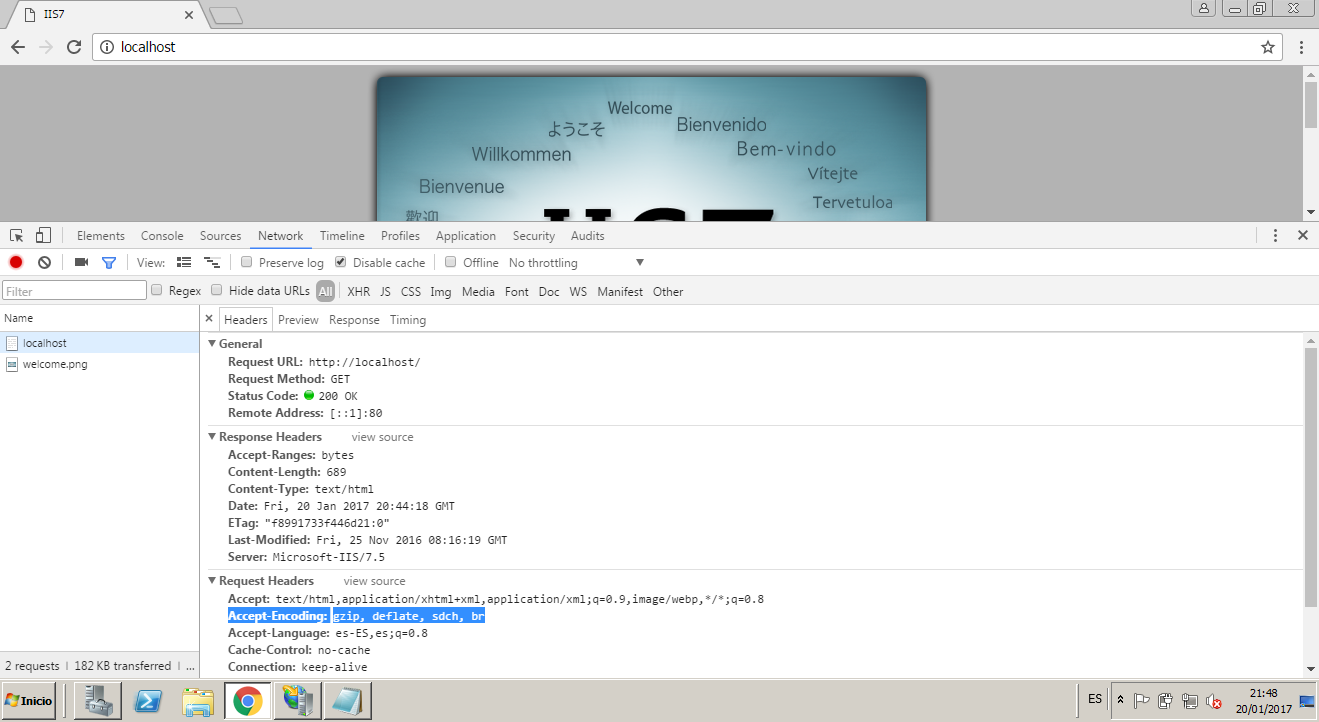
\includegraphics[width=14.7cm]{./img/ejercicio5_3.png} 	
	\caption{Windows, Accept-Enconding.} \label{fig:ejercicio5_3}
\end{figure}

\begin{figure}[H] 
	\centering
	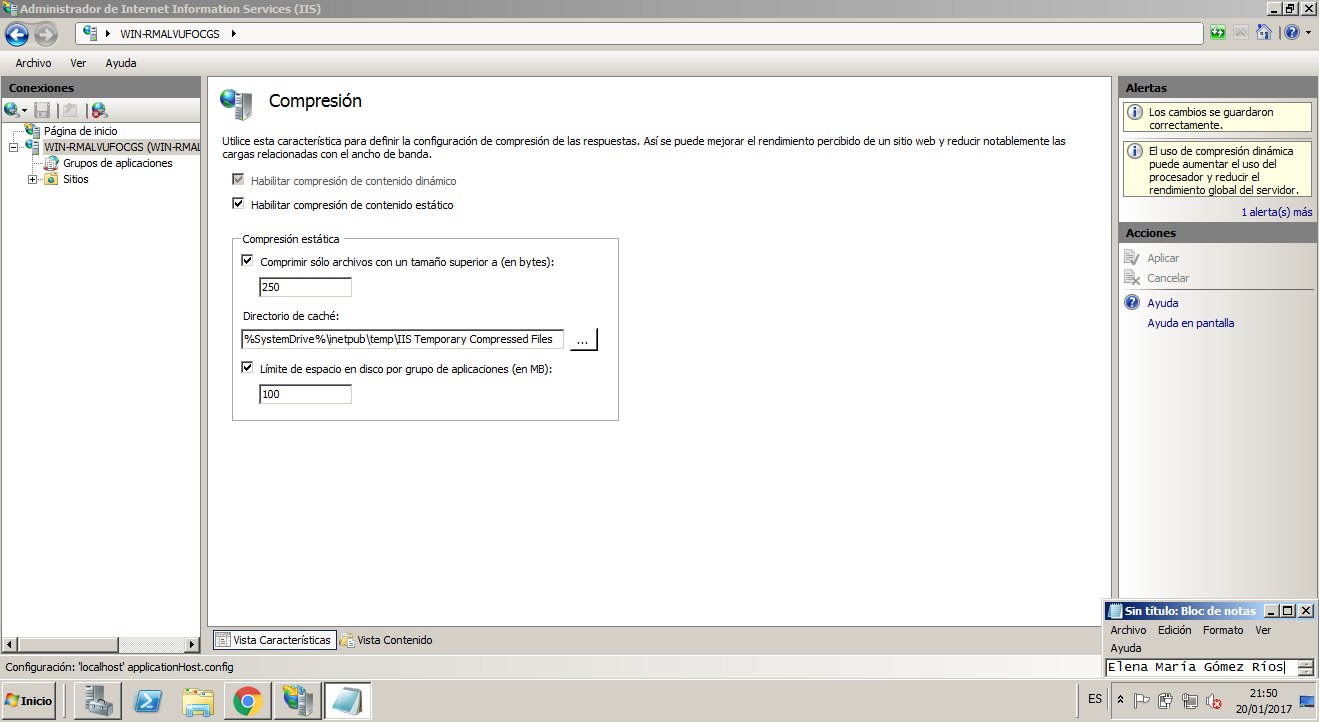
\includegraphics[width=14.7cm]{./img/ejercicio5_4.png} 	
	\caption{Windows, cambio en la configuración de compresión.} \label{fig:ejercicio5_4}
\end{figure}

\begin{figure}[H] 
	\centering
	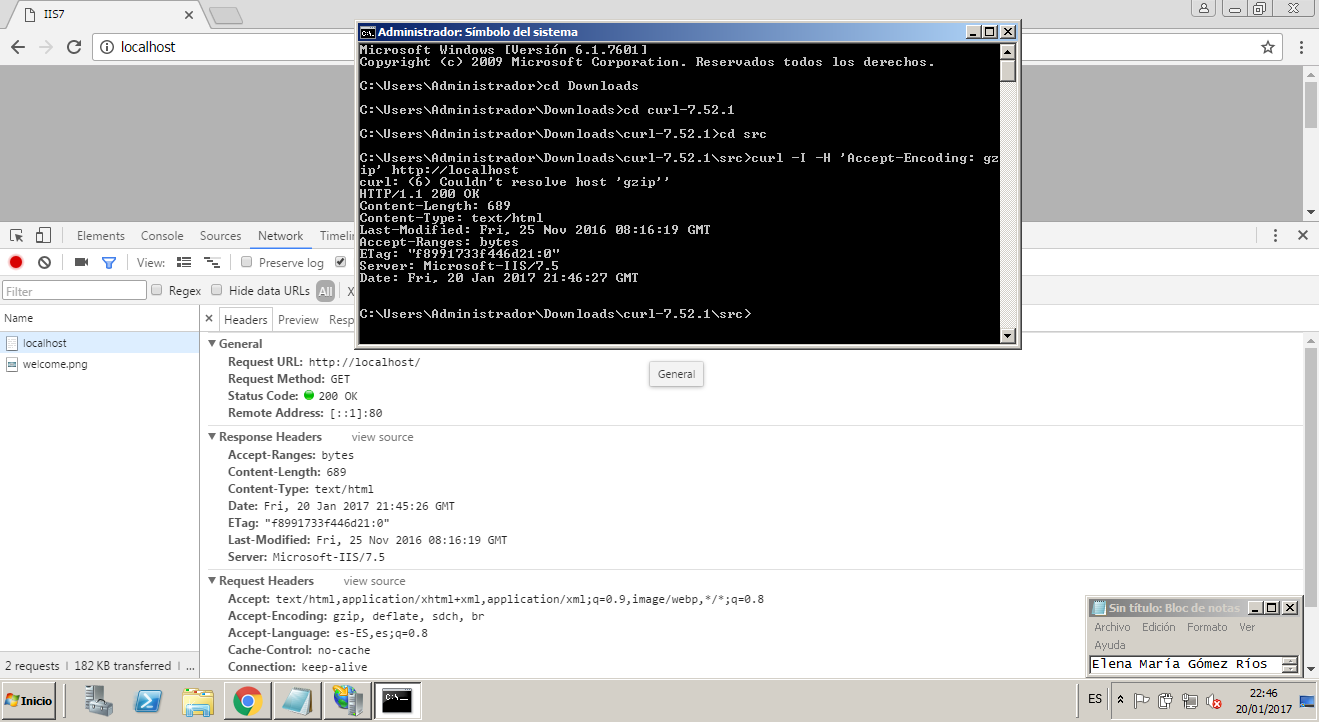
\includegraphics[width=14.7cm]{./img/ejercicio5_5.png} 	
	\caption{Windows, curl.} \label{fig:ejercicio5_5}
\end{figure}


%----------------------------------------------------------------------------------------
%  Cuestión 6:
%----------------------------------------------------------------------------------------

\section{Cuestión 6:}

\subsection{a) Elija un servicio (el que usted quiera) y modifique un parámetro para mejorar su comportamiento.}

\subsection{b) Monitorice el servicio antes y después de la modificación del parámetro aplicando cargas al sistema (antes y después) mostrando los resultados de la monitorización.}

He probado a mejorar el servicio httpd cambiando la variable MaxKeepAliveRequests que indica el 
número máximo de clientes que pueden acceder al servidor. Hemos fijado dicha variable 
primero a 150, su valor por defecto, y más tarde a 500, y hemos comprobado en ambos casos 
cuánto tarda ab en mandar 1000 peticiones de 200 en 200. Los resultados con la variable a 150 
han sido los de la figura \ref{fig:ejercicio6_1}. Los resultados con la variable a 500 han sido los de la figura \ref{fig:ejercicio6_2}. Vemos, sin embargo, que los tiempos empeoran notablemente.
 
\begin{figure}[H] 
	\centering
	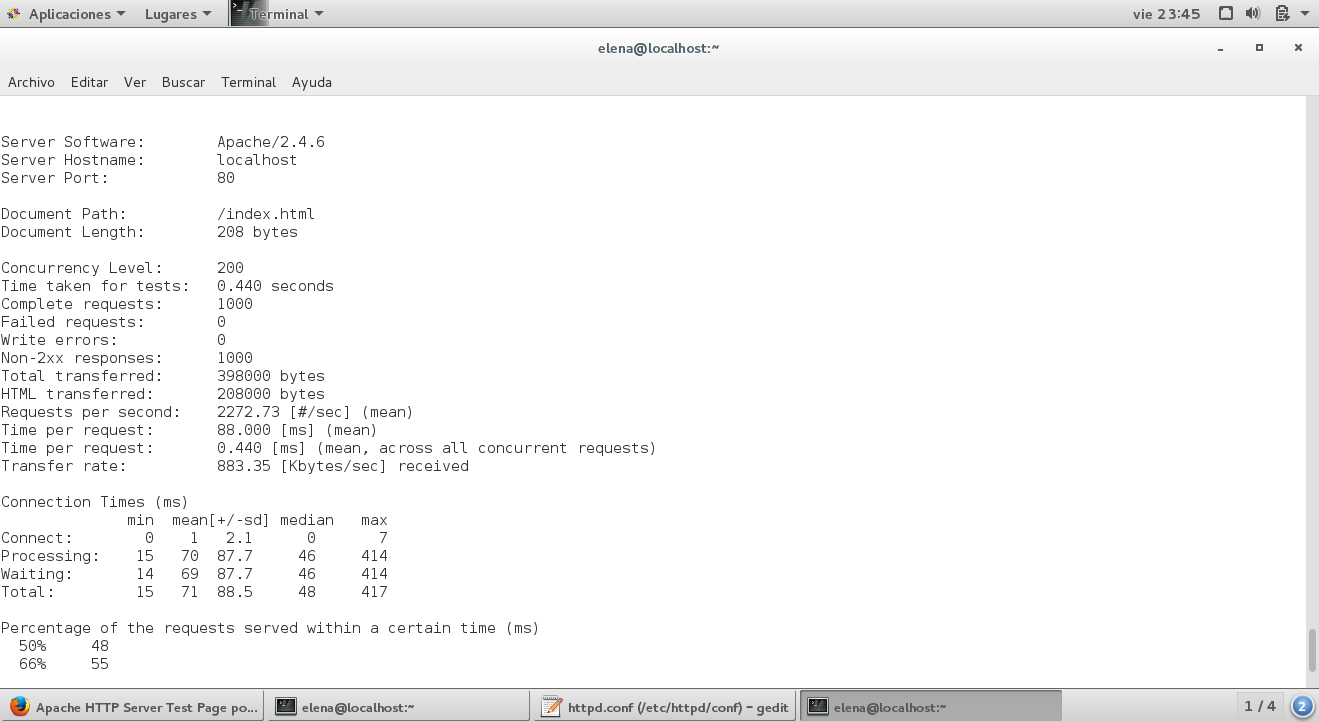
\includegraphics[width=14.7cm]{./img/ejercicio6_1.png} 	
	\caption{Windows, ab.} \label{fig:ejercicio6_1}
\end{figure}



\begin{figure}[H] 
	\centering
	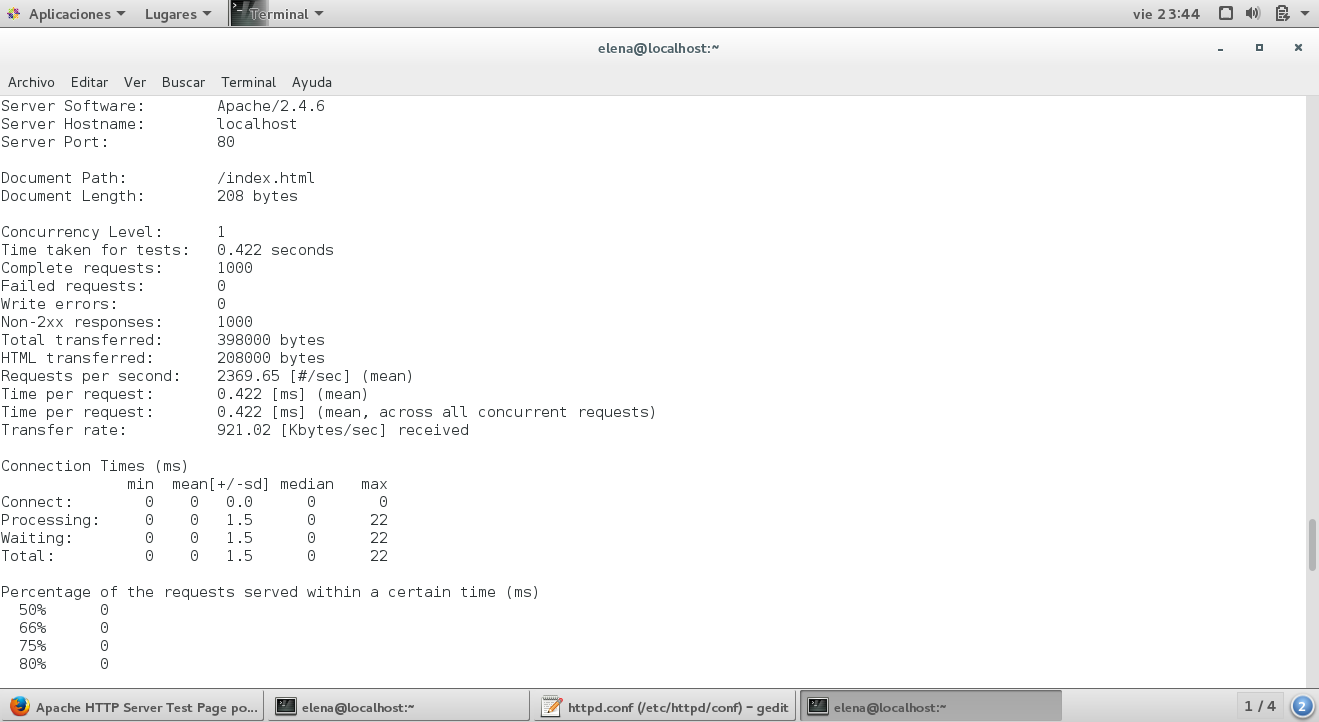
\includegraphics[width=14.7cm]{./img/ejercicio6_2.png} 	
	\caption{Windows, ab.} \label{fig:ejercicio6_2}
\end{figure}



%------------------------------------------------

\bibliography{citas} %archivo citas.bib que contiene las entradas 
\bibliographystyle{plain} % hay varias formas de citar

\end{document}
